% 若编译失败,且生成 .synctex(busy) 辅助文件,可能有两个原因:
% 1. 需要插入的图片不存在:Ctrl + F 搜索 'figure' 将这些代码注释/删除掉即可
% 2. 路径/文件名含中文或空格:更改路径/文件名即可

% ------------------------------------------------------------- %
% >> ------------------ 文章宏包及相关设置 ------------------ << %
% 设定文章类型与编码格式
    \documentclass[UTF8]{report}		

% 本文特殊宏包
    \usepackage{siunitx} % 埃米单位

% 本文的特殊宏定义
\def\Im{\mathrm{\,Im\,}}
\def\Re{\mathrm{\,Re\,}}
\def\Ln{\mathrm{\,Ln\,}}
\def\Arg{\mathrm{\,Arg\,}}
\def\Arccos{\mathrm{\,Arccos\,}}
\def\Arcsin{\mathrm{\,Arcsin\,}}
\def\Arctan{\mathrm{\,Arctan\,}}

% 通用宏定义
\def\N{\mathbb{N}}
\def\F{\mathbb{F}}
\def\Z{\mathbb{Z}}
\def\Q{\mathbb{Q}}
\def\R{\mathbb{R}}
\def\C{\mathbb{C}}
\def\T{\mathbb{T}}
\def\S{\mathbb{S}}
\def\A{\mathbb{A}}
\def\I{\mathscr{I}}
\def\d{\mathrm{d}}
\def\p{\partial}


% 导入基本宏包
    \usepackage[UTF8]{ctex}     % 设置文档为中文语言
    \usepackage[colorlinks, linkcolor=blue, anchorcolor=blue, citecolor=blue, urlcolor=blue]{hyperref}  % 宏包:自动生成超链接 (此宏包与标题中的数学环境冲突)
    % \usepackage{docmute}    % 宏包:子文件导入时自动去除导言区,用于主/子文件的写作方式,\include{./51单片机笔记}即可。注:启用此宏包会导致.tex文件capacity受限。
    \usepackage{amsmath}    % 宏包:数学公式
    \usepackage{mathrsfs}   % 宏包:提供更多数学符号
    \usepackage{amssymb}    % 宏包:提供更多数学符号
    \usepackage{pifont}     % 宏包:提供了特殊符号和字体
    \usepackage{extarrows}  % 宏包:更多箭头符号
    \usepackage{multicol}   % 宏包:支持多栏 
    \usepackage{graphicx}   % 宏包:插入图片
    \usepackage{float}      % 宏包:设置图片浮动位置
    \usepackage{mathtools}  % 宏包:数学公式
    %\usepackage{article}    % 宏包:使文本排版更加优美
    %\usepackage{tikz}       % 宏包:绘图工具
    %\usepackage{pgfplots}   % 宏包:绘图工具

% 文章页面margin设置
    \usepackage[a4paper]{geometry}
        \geometry{top=1in}  % 1 inch= 2.46 cm, 0.75 inch = 1.85 cm
        \geometry{bottom=1in}
        \geometry{left=0.75in}
        \geometry{right=0.75in}   % 设置上下左右页边距
        \geometry{marginparwidth=1.75cm}    % 设置边注距离(注释、标记等)

% 配置数学环境
    \usepackage{amsthm} % 宏包:数学环境配置
    % theorem-line 环境自定义
        \newtheoremstyle{MyLineTheoremStyle}% <name>
            {11pt}% <space above>
            {11pt}% <space below>
            {}% <body font> 使用默认正文字体
            {}% <indent amount>
            {\bfseries}% <theorem head font> 设置标题项为加粗
            {:}% <punctuation after theorem head>
            {.5em}% <space after theorem head>
            {\textbf{#1}\thmnumber{#2}\ \ (\,\textbf{#3}\,)}% 设置标题内容顺序
        \theoremstyle{MyLineTheoremStyle} % 应用自定义的定理样式
        \newtheorem{LineTheorem}{Theorem.\,}
    % theorem-block 环境自定义
        \newtheoremstyle{MyBlockTheoremStyle}% <name>
            {11pt}% <space above>
            {11pt}% <space below>
            {}% <body font> 使用默认正文字体
            {}% <indent amount>
            {\bfseries}% <theorem head font> 设置标题项为加粗
            {:\\ \indent}% <punctuation after theorem head>
            {.5em}% <space after theorem head>
            {\textbf{#1}\thmnumber{#2}\ \ (\,\textbf{#3}\,)}% 设置标题内容顺序
        \theoremstyle{MyBlockTheoremStyle} % 应用自定义的定理样式
        \newtheorem{BlockTheorem}[LineTheorem]{Theorem.\,} % 使用 LineTheorem 的计数器
    % definition 环境自定义
        \newtheoremstyle{MySubsubsectionStyle}% <name>
            {11pt}% <space above>
            {11pt}% <space below>
            {}% <body font> 使用默认正文字体
            {}% <indent amount>
            {\bfseries}% <theorem head font> 设置标题项为加粗
            {:\\ \indent}% <punctuation after theorem head>
            {0pt}% <space after theorem head>
            {\textbf{#3}}% 设置标题内容顺序
        \theoremstyle{MySubsubsectionStyle} % 应用自定义的定理样式
        \newtheorem{definition}{}

%宏包:有色文本框(proof环境)及其设置
    \usepackage[dvipsnames,svgnames]{xcolor}    %设置插入的文本框颜色
    \usepackage[strict]{changepage}     % 提供一个 adjustwidth 环境
    \usepackage{framed}     % 实现方框效果
        \definecolor{graybox_color}{rgb}{0.95,0.95,0.96} % 文本框颜色。修改此行中的 rgb 数值即可改变方框纹颜色,具体颜色的rgb数值可以在网站https://colordrop.io/ 中获得。(截止目前的尝试还没有成功过,感觉单位不一样)(找到喜欢的颜色,点击下方的小眼睛,找到rgb值,复制修改即可)
        \newenvironment{graybox}{%
        \def\FrameCommand{%
        \hspace{1pt}%
        {\color{gray}\small \vrule width 2pt}%
        {\color{graybox_color}\vrule width 4pt}%
        \colorbox{graybox_color}%
        }%
        \MakeFramed{\advance\hsize-\width\FrameRestore}%
        \noindent\hspace{-4.55pt}% disable indenting first paragraph
        \begin{adjustwidth}{}{7pt}%
        \vspace{2pt}\vspace{2pt}%
        }
        {%
        \vspace{2pt}\end{adjustwidth}\endMakeFramed%
        }

% 外源代码插入设置
    % matlab 代码插入设置
    %\usepackage{matlab-prettifier}
    %    \lstset{
    %        style=Matlab-editor,  % 继承matlab代码颜色等
    %    }
    %\usepackage[most]{tcolorbox} % 引入tcolorbox包 
    %\usepackage{listings} % 引入listings包
    %    \tcbuselibrary{listings, skins, breakable}
    %    \newfontfamily\codefont{Consolas} % 定义需要的 codefont 字体
    %    \lstdefinestyle{matlabstyle}{
    %        language=Matlab,
    %        basicstyle=\small\ttfamily\codefont,    % ttfamily 确保等宽 
    %        breakatwhitespace=false,
    %        breaklines=true,
    %        captionpos=b,
    %        keepspaces=true,
    %        numbers=left,
    %        numbersep=15pt,
    %        showspaces=false,
    %        showstringspaces=false,
    %        showtabs=false,
    %        tabsize=2
    %    }
    %    \newtcblisting{matlablisting}{
    %        arc=2pt,        % 圆角半径
    %        top=-5pt,
    %        bottom=-5pt,
    %        left=1mm,
    %        listing only,
    %        listing style=matlabstyle,
    %        breakable,
    %        colback=white   % 选一个合适的颜色
    %    }
% table 支持
    \usepackage{booktabs}   % 宏包:三线表
    \usepackage{tabularray} % 宏包:表格排版
    \usepackage{longtable}  % 宏包:长表格


%figure 设置
%    \usepackage{graphicx}  % 支持 jpg, png, eps, pdf 图片 
%    \usepackage{svg}       % 支持 svg 图片
%        \svgsetup{
%             指向 inkscape.exe 的路径
%            inkscapeexe = C:/aa_MySame/inkscape/bin/inkscape.exe, 
%            inkscapeexe = C:/aa_MySame/inkscape/bin/inkscape.exe, 
%             一定程度上修复导入后图片文字溢出几何图形的问题
%            inkscapelatex = false                 
%        }
%    \usepackage{subcaption} % subfigure 子图支持

%图表进阶设置
%    \usepackage{caption}    % 图注、表注
%        \captionsetup[figure]{name=图}  
%        \captionsetup[table]{name=表}
%        \captionsetup{labelfont=bf, font=small}
%    \usepackage{float}     % 图表位置浮动设置 

% 圆圈序号自定义
    \newcommand*\circled[1]{\tikz[baseline=(char.base)]{\node[shape=circle,draw,inner sep=0.8pt, line width = 0.03em] (char) {\small \bfseries #1};}}   % TikZ solution

% 列表设置
%    \usepackage{enumitem}   % 宏包:列表环境设置
%        \setlist[enumerate]{itemsep=0pt, parsep=0pt, topsep=0pt, partopsep=0pt, leftmargin=3.5em} 
%        \setlist[itemize]{itemsep=0pt, parsep=0pt, topsep=0pt, partopsep=0pt, leftmargin=3.5em}
%        \newlist{circledenum}{enumerate}{1} % 创建一个新的枚举环境  
%        \setlist[circledenum,1]{  
%            label=\protect\circled{\arabic*}, % 使用 \arabic* 来获取当前枚举计数器的值,并用 \circled 包装它  
%            ref=\arabic*, % 如果需要引用列表项,这将决定引用格式(这里仍然使用数字)
%            itemsep=0pt, parsep=0pt, topsep=0pt, partopsep=0pt, leftmargin=3.5em
%        }  

% 其它设置
    % 脚注设置
        \renewcommand\thefootnote{\ding{\numexpr171+\value{footnote}}}
    % 参考文献引用设置
        \bibliographystyle{unsrt}   % 设置参考文献引用格式为unsrt
        \newcommand{\upcite}[1]{\textsuperscript{\cite{#1}}}     % 自定义上角标式引用
    % 文章序言设置
        \newcommand{\cnabstractname}{序言}
        \newenvironment{cnabstract}{%
            \par\Large
            \noindent\mbox{}\hfill{\bfseries \cnabstractname}\hfill\mbox{}\par
            \vskip 2.5ex
            }{\par\vskip 2.5ex}

% 文章默认字体设置
    \usepackage{fontspec}   % 宏包:字体设置
        \setmainfont{SimSun}    % 设置中文字体为宋体字体
        \setCJKmainfont[AutoFakeBold=3]{SimSun} % 设置加粗字体为 SimSun 族,AutoFakeBold 可以调整字体粗细
        \setmainfont{Times New Roman} % 设置英文字体为Times New Roman

% 各级标题自定义设置
    \usepackage{titlesec}   
        \titleformat{\chapter}[hang]{\normalfont\huge\bfseries\centering}{第\,\thechapter\,章}{20pt}{}
        \titlespacing*{\chapter}{0pt}{-20pt}{20pt} % 控制上方空白的大小
        % section标题自定义设置 
        \titleformat{\section}[hang]{\normalfont\Large\bfseries}{§\,\thesection\,}{8pt}{}
        % subsubsection标题自定义设置
        %\titleformat{\subsubsection}[hang]{\normalfont\bfseries}{}{8pt}{}

% >> ------------------ 文章宏包及相关设置 ------------------ << %
% ------------------------------------------------------------- %

% ----------------------------------------------------------- %
% >> --------------------- 文章信息区 --------------------- << %
% 页眉页脚设置
    \usepackage{fancyhdr}   %宏包:页眉页脚设置
        \pagestyle{fancy}
        \fancyhf{}
        \cfoot{\thepage}
        \renewcommand\headrulewidth{1pt}
        \renewcommand\footrulewidth{0pt}
        \lhead{2024.8 -- 2025.1} 
        \chead{yinchao050313@gmail.com}    
        \rhead{yinchao23@mails.ucas.ac.cn}
%文档信息设置
    \title{原子物理\\Atomic Physics}
    \author{尹超\\ \footnotesize 中国科学院大学,北京 100049\\ Carter Yin \\ \footnotesize University of Chinese Academy of Sciences, Beijing 100049, China}
    \date{\footnotesize 2024.8 -- 2025.1}
% >> --------------------- 文章信息区 --------------------- << %
% ----------------------------------------------------------- %

% 开始编辑文章

\begin{document} 
\zihao{5}             % 设置全文字号大小, -4 为小四, 5 为五号

% --------------------------------------------------------------- %
% >> --------------------- 封面序言与目录 --------------------- << %
% 封面
    \maketitle\newpage  
    \pagenumbering{Roman} % 页码为大写罗马数字
    \thispagestyle{fancy}   % 显示页码、页眉等

% 序言
    \begin{cnabstract}\normalsize 
        本笔记为原子物理的笔记整理\par
        讲课教师:\par
        • 李海波\par 
        • 办公室: ⾼能物理所 多学科⼤楼 619\par
        • telephone: 88233203\par
        • email: lihb@ihep.ac.cn\par
        助教:\par
        • 胡海明 研究员 中科院高能物理所 \par
        • 办公室: ⾼能物理所 多学科⼤楼 519\par
        • telephone: 18811590054\par
        • email:huhm@ihep.ac.cn
\end{cnabstract}    
\addcontentsline{toc}{chapter}{序言} % 手动添加为目录

% 目录
    \setcounter{tocdepth}{4}                % 目录深度(为1时显示到section)
    \tableofcontents                        % 目录页
    \addcontentsline{toc}{chapter}{目录}    % 手动添加此页为目录
    \thispagestyle{fancy}                   % 显示页码、页眉等 

% 收尾工作
    \newpage    
    \pagenumbering{arabic} 


% >> --------------------- 封面序言与目录 --------------------- << %
% --------------------------------------------------------------- %


\chapter{卢瑟福原子模型}\thispagestyle{fancy} 
\section{Avogadro's Number}
\begin{definition}[Avogadro's Number]
    • Avogadro's number is the number of atoms in 12 grams of carbon-12, which is equal to \(6.022 \times 10^{23}\) \par
    • The number of atoms in 1 gram of hydrogen is \(6.022 \times 10^{23}\) \par
    • The number of atoms in 1 gram of any element is \(6.022 \times 10^{23}\) \par
    • The number of atoms in 1 mole of any element is \(6.022 \times 10^{23}\) \par
\end{definition}



\begin{definition}[原子单位u]
    • 原子单位是一种质量单位,定义为碳-12的原子质量的1/12,等于 \(1.66053906660 \times 10^{-27}\) 千克 \par
    • 1u = \(1.66053906660 \times 10^{-27}\) kg \par
    • 1u = \(931.49410242\) MeV/c\(^2\) \par
    • 1u = \(1.66053906660 \times 10^{-24}\) g \par
    • 1u = \(1.66053906660 \times 10^{-3}\) amu \par
\end{definition}

\begin{definition}[普适气体常数]
    • 普适气体常数 \(R = 8.314462618\) J/(mol·K) \par
    • 普适气体常数 \(R = 0.08205736608\) L·atm/(mol·K) \par
    • 普适气体常数 \(R = 62.3635777483\) L·Torr/(mol·K) \par
    与玻尔兹曼常数的关系:\(R = N_A k_B\) \par
    \end{definition}

    \begin{definition}[原子大小的一种简单估计]
        对任意一种原子 \( \prescript{A}{}{X}\), \( A \) 克含有 \( N_A \) 个 \( \prescript{A}{}{X}\) 原子,假定其密度为 \( \rho \),又假定原子是球形的,半径为 \( r \),每个原子占有体积为 \( \frac{4}{3}\pi r^3 \),则有
        \[
        r=\left(\frac{3A}{4 \pi \rho N_{A}}\right)^{1 / 3}
        \]
    \end{definition}

\begin{definition}[常见粒子的半径]
    原子半径:\(r \approx 0.1 \, \text{nm}\) \par
    原子核半径:\(r \approx 1 \times 10^{-15} \, \text{m}\) \par
    质子半径:\(r \approx 0.8 \times 10^{-15} \, \text{m}\) \par
    电子半径:\(r \approx 2.8 \times 10^{-15} \, \text{m}\) \par
\end{definition}

\section{gaige-masidun实验}

\begin{definition}[盖革-马斯顿实验]
    与汤姆孙模型的矛盾:\par
    • 汤姆孙模型认为原子是一个带正电的均匀球体,电子均匀分布在球体内部,但是这样的模型无法解释原子的稳定性。\par
    • 盖革-马斯顿实验:\par
    • 1911年,盖革-马斯顿实验,利用 \(\alpha\) 粒子轰击金箔,发现 \(\alpha\) 粒子的散射角度与金箔厚度不符合汤姆孙模型的预期。\par
    • 实验结果:\par
    • 大部分 \(\alpha\) 粒子直接穿透金箔,少部分 \(\alpha\) 粒子被散射,极少数 \(\alpha\) 粒子被反射。\par
    • 结论:\par
    • 原子核半径 \(r \approx 1 \times 10^{-15} \, \text{m}\) \par
    • 原子核带正电,电子绕核运动 \par
\end{definition}

\section{汤姆孙模型和卢瑟福模型}

\begin{definition}[汤姆孙模型的困难]
    电子绕核运动,会受到库仑力,会加速,加速的电子会发射辐射,失去能量,最终会坠入核。\par
    对于汤姆逊模型而言,只有掠入射(\(r=R\))时,入射α粒子受力最大,设为 \(F_{\text{max}}\),我们来看看此条件下α粒子的最大偏转角是多少?\par
    \begin{figure}[ht]
        \centering
        \includegraphics[width=1\textwidth]{C:/Users/78003/Desktop/ap/1.png}
        \caption{\textbf{1}}
        \label{fig:1}
    \end{figure}
    \begin{figure}[ht]
        \centering
        \includegraphics[width=0.8\textwidth]{C:/Users/78003/Desktop/ap/2.png}
        \caption{\textbf{2}}
        \label{fig:2}
    \end{figure}
    \begin{figure}[ht]
        \centering
        \includegraphics[width=0.9\textwidth]{C:/Users/78003/Desktop/ap/3.png}
        \caption{\textbf{3}}
        \label{fig:3}
    \end{figure}
    \begin{figure}[ht]
        \centering
        \includegraphics[width=0.6\textwidth]{C:/Users/78003/Desktop/ap/4.png}
        \caption{\textbf{4}}
        \label{fig:4}
    \end{figure}
    \begin{figure}[ht]
        \centering
        \includegraphics[width=1\textwidth]{C:/Users/78003/Desktop/ap/5.png}
        \caption{\textbf{5}}
        \label{fig:5}
    \end{figure}
    \begin{figure}[ht]
        \centering
        \includegraphics[width=1\textwidth]{C:/Users/78003/Desktop/ap/6.png}
        \caption{\textbf{6}}
        \label{fig:6}
    \end{figure}

    \begin{figure}[ht]
        \centering
        \includegraphics[width=1\textwidth]{C:/Users/78003/Desktop/ap/r1.png}
        \caption{\textbf{r1}}
        \label{fig:r1}
    \end{figure}
    \begin{figure}[ht]
        \centering
        \includegraphics[width=1\textwidth]{C:/Users/78003/Desktop/ap/r2.png}
        \caption{\textbf{r2}}
        \label{fig:r2}
    \end{figure}
    \begin{figure}[ht]
        \centering
        \includegraphics[width=1\textwidth]{C:/Users/78003/Desktop/ap/r3.png}
        \caption{\textbf{r3}}
        \label{fig:r3}
    \end{figure}
    \begin{figure}[ht]
        \centering
        \includegraphics[width=1\textwidth]{C:/Users/78003/Desktop/ap/r4.png}
        \caption{\textbf{r4}}
        \label{fig:r4}
    \end{figure}
    \begin{figure}[ht]
        \centering
        \includegraphics[width=1\textwidth]{C:/Users/78003/Desktop/ap/c1.png}
        \caption{\textbf{c1}}
        \label{fig:c1}
    \end{figure}
    \begin{figure}[ht]
        \centering
        \includegraphics[width=1\textwidth]{C:/Users/78003/Desktop/ap/c2.png}
        \caption{\textbf{c2}}
        \label{fig:c2}
    \end{figure}
    \begin{figure}[ht]
        \centering
        \includegraphics[width=1\textwidth]{C:/Users/78003/Desktop/ap/c3.png}
        \caption{\textbf{c3}}
        \label{fig:c3}
    \end{figure}
    \begin{figure}[ht]
        \centering
        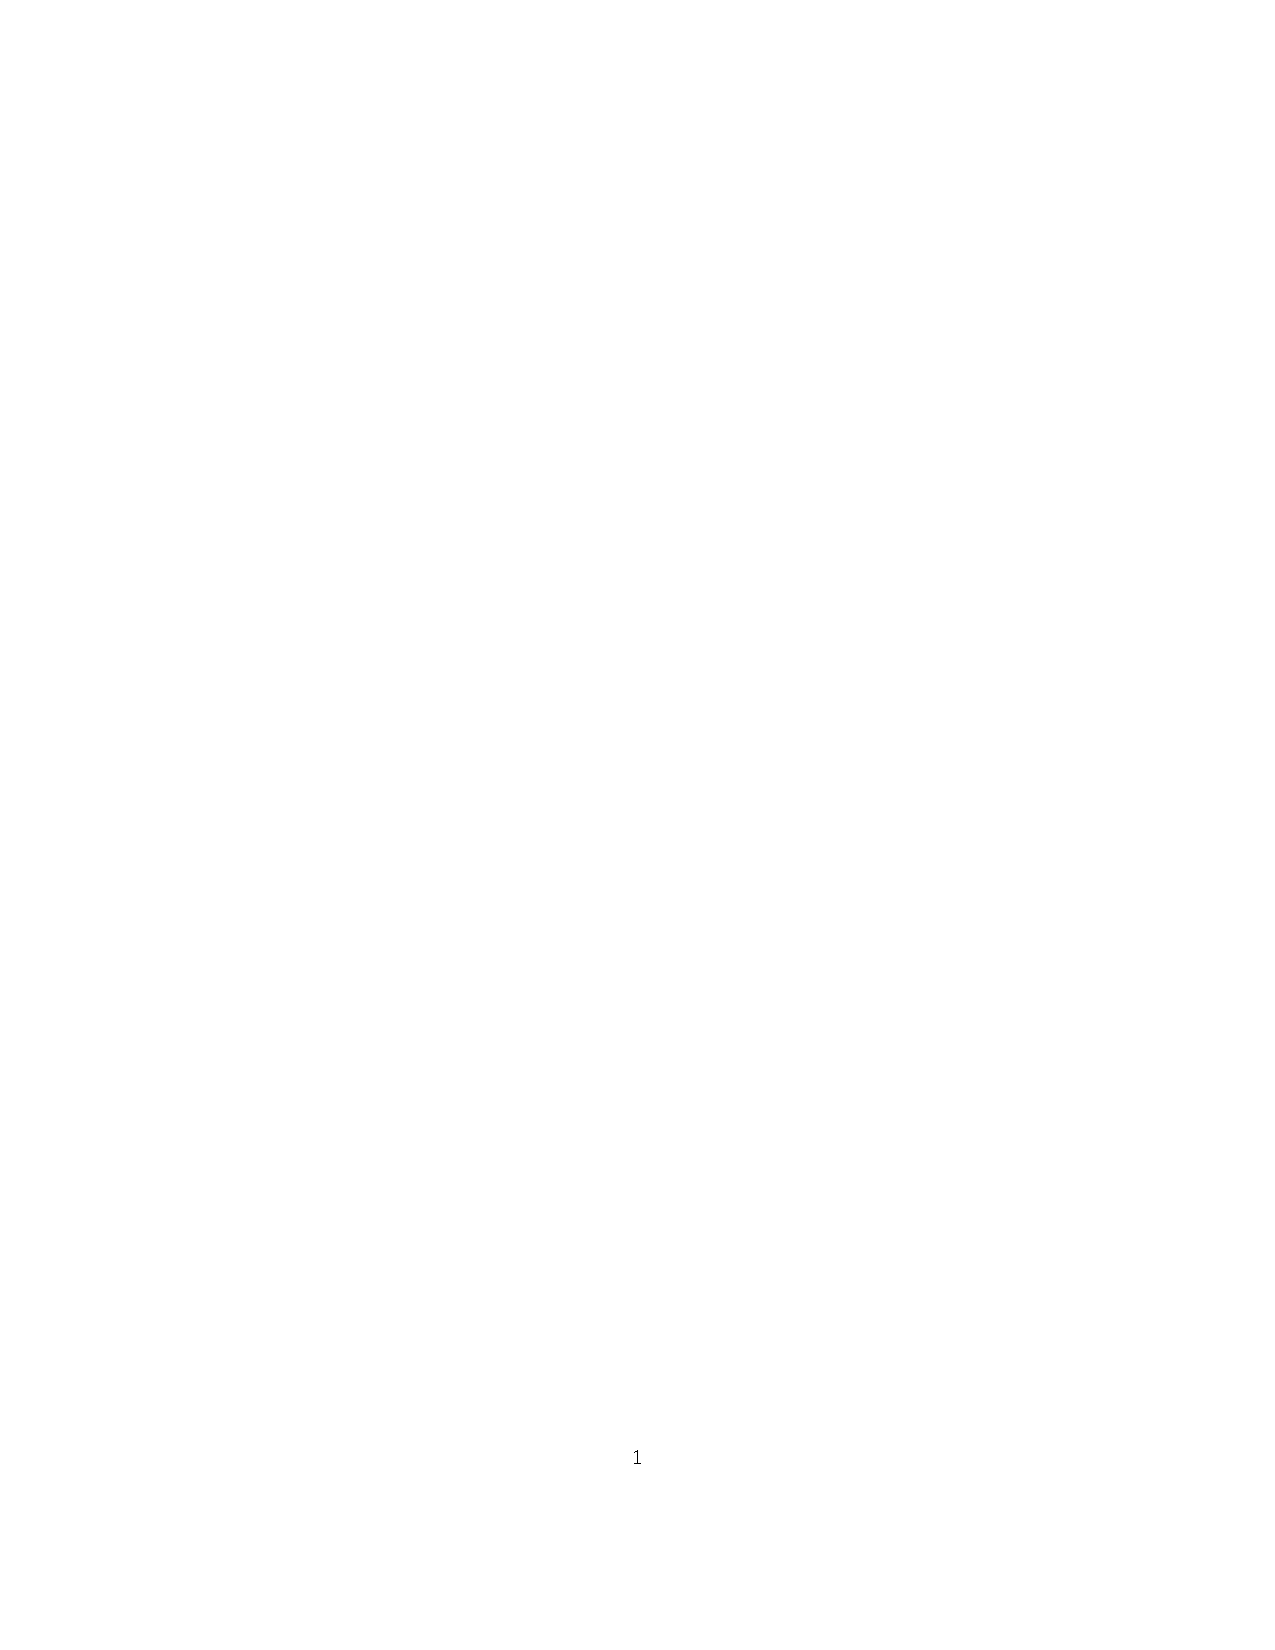
\includegraphics[width=1\textwidth]{C:/Users/78003/Desktop/ap/c4.png}
        \caption{\textbf{c4}}
        \label{fig:c4}
    \end{figure}
    \begin{figure}[ht]
        \centering
        \includegraphics[width=1\textwidth]{C:/Users/78003/Desktop/ap/c5.png}
        \caption{\textbf{c5}}
        \label{fig:c5}
    \end{figure}
    \begin{figure}[ht]
        \centering
        \includegraphics[width=1\textwidth]{C:/Users/78003/Desktop/ap/c6.png}
        \caption{\textbf{c6}}
        \label{fig:c6}
    \end{figure}
    \begin{figure}[ht]
        \centering
        \includegraphics[width=1\textwidth]{C:/Users/78003/Desktop/ap/c7.png}
        \caption{\textbf{c7}}
        \label{fig:c7}
    \end{figure}
    \begin{figure}[ht]
        \centering
        \includegraphics[width=1\textwidth]{C:/Users/78003/Desktop/ap/rg1.png}
        \caption{\textbf{rg1}}
        \label{fig:rg1}
    \end{figure}
    \begin{figure}[ht]
        \centering
        \includegraphics[width=1\textwidth]{C:/Users/78003/Desktop/ap/rg2.png}
        \caption{\textbf{rg2}}
        \label{fig:rg2}
    \end{figure}
    \begin{figure}[ht]
        \centering
        \includegraphics[width=1\textwidth]{C:/Users/78003/Desktop/ap/rg3.png}
        \caption{\textbf{rg3}}
        \label{fig:rg3}
    \end{figure}
    \begin{figure}[ht]
        \centering
        \includegraphics[width=1\textwidth]{C:/Users/78003/Desktop/ap/rg4.png}
        \caption{\textbf{rg4}}
        \label{fig:rg4}
    \end{figure}
    \begin{figure}[ht]
        \centering
        \includegraphics[width=1\textwidth]{C:/Users/78003/Desktop/ap/sy1.png}
        \caption{\textbf{sy1}}
        \label{fig:sy1}
    \end{figure}
    \begin{figure}[ht]
        \centering
        \includegraphics[width=1\textwidth]{C:/Users/78003/Desktop/ap/sy2.png}
        \caption{\textbf{sy2}}
        \label{fig:sy2}
    \end{figure}
    \begin{figure}[ht]
        \centering
        \includegraphics[width=1\textwidth]{C:/Users/78003/Desktop/ap/sy3.png}
        \caption{\textbf{sy3}}
        \label{fig:sy3}
    \end{figure}
    \begin{figure}[ht]
        \centering
        \includegraphics[width=1\textwidth]{C:/Users/78003/Desktop/ap/xt1.png}
        \caption{\textbf{xt1}}
        \label{fig:xt1}
    \end{figure}
    \begin{figure}[ht]
        \centering
        \rotatebox{270}{\includegraphics[width=1.3\textwidth]{C:/Users/78003/Desktop/ap/sx1.png}}
        \caption{\textbf{sx1}}
        \label{fig:sx1}
    \end{figure}
    \begin{figure}[ht]
        \centering
        \rotatebox{270}{\includegraphics[width=1.3\textwidth]{C:/Users/78003/Desktop/ap/sx2.png}}
        \caption{\textbf{sx2}}
        \label{fig:sx2}
    \end{figure}
    \begin{figure}[ht]
        \centering
        \rotatebox{270}{\includegraphics[width=1.3\textwidth]{C:/Users/78003/Desktop/ap/sx3.png}}
        \caption{\textbf{sx3}}
        \label{fig:sx3}
    \end{figure}
    \begin{figure}[ht]
        \centering
        \includegraphics[width=1\textwidth]{C:/Users/78003/Desktop/ap/sx4.png}
        \caption{\textbf{sx4}}
        \label{fig:sx4}
    \end{figure}
    \begin{figure}[ht]
        \centering
        \includegraphics[width=1\textwidth]{C:/Users/78003/Desktop/ap/xt2.png}
        \caption{\textbf{xt2}}
        \label{fig:xt2}
    \end{figure}
    \begin{figure}[ht]
        \centering
        \includegraphics[width=1\textwidth]{C:/Users/78003/Desktop/ap/sm1.png}
        \caption{\textbf{sm1}}
        \label{fig:sm1}
    \end{figure}
    \begin{figure}[ht]
        \centering
        \includegraphics[width=1\textwidth]{C:/Users/78003/Desktop/ap/sm2.png}
        \caption{\textbf{sm2}}
        \label{fig:sm2}
    \end{figure}
    \begin{figure}[ht]
        \centering
        \includegraphics[width=1\textwidth]{C:/Users/78003/Desktop/ap/bg1.png}
        \caption{\textbf{bg1}}
        \label{fig:bg1}
    \end{figure}
    \begin{figure}[ht]
        \centering
        \includegraphics[width=1\textwidth]{C:/Users/78003/Desktop/ap/est1.png}
        \caption{\textbf{est1}}
        \label{fig:est1}
    \end{figure}
    \begin{figure}[ht]
        \centering
        \includegraphics[width=1\textwidth]{C:/Users/78003/Desktop/ap/est2.png}
        \caption{\textbf{est2}}
        \label{fig:est2}
    \end{figure}
    \begin{figure}[ht]
        \centering
        \includegraphics[width=1\textwidth]{C:/Users/78003/Desktop/ap/q1.png}
        \caption{\textbf{q1}}
        \label{fig:q1}
    \end{figure}
    \begin{figure}[ht]
        \centering
        \includegraphics[width=1\textwidth]{C:/Users/78003/Desktop/ap/q2.png}
        \caption{\textbf{q2}}
        \label{fig:q2}
    \end{figure}
\end{definition}

\chapter{原子的量子态:玻尔模型}\thispagestyle{fancy} 
\section{background knowledge}
\begin{figure}[ht]
    \centering
    \includegraphics[width=0.8\textwidth]{C:/Users/78003/Desktop/ap/back1.png}
    \caption{\textbf{back1}}
    \label{fig:back1}
\end{figure}
\begin{figure}[ht]
    \centering
    \includegraphics[width=0.8\textwidth]{C:/Users/78003/Desktop/ap/back2.png}
    \caption{\textbf{back2}}
    \label{fig:back2}
\end{figure}
\begin{figure}[ht]
    \centering
    \includegraphics[width=1\textwidth]{C:/Users/78003/Desktop/ap/back3.png}
    \caption{\textbf{back3}}
    \label{fig:back3}
\end{figure}
\begin{figure}[ht]
    \centering
    \includegraphics[width=1\textwidth]{C:/Users/78003/Desktop/ap/back4.png}
    \caption{\textbf{back4}}
    \label{fig:back4}
\end{figure}

\cleardoublepage
\section{黑体定义}

\begin{figure}[ht]
    \centering
    \includegraphics[width=1\textwidth]{C:/Users/78003/Desktop/ap/ht1.png}
    \caption{\textbf{ht1}}
    \label{fig:ht1}
\end{figure}

\cleardoublepage
\section{基尔霍夫定律}

\begin{figure}[ht]
    \centering
    \includegraphics[width=1\textwidth]{C:/Users/78003/Desktop/ap/kir1.png}
    \caption{\textbf{kir1}}
    \label{fig:kir1}
\end{figure}

\begin{figure}[ht]
    \centering
    \includegraphics[width=1\textwidth]{C:/Users/78003/Desktop/ap/kir2.png}
    \caption{\textbf{kir2}}
    \label{fig:kir2}
\end{figure}

\cleardoublepage
\section{黑体辐射定律}

\begin{figure}[ht]
    \centering
    \includegraphics[width=1\textwidth]{C:/Users/78003/Desktop/ap/bb1.png}
    \caption{\textbf{bb1}}
    \label{fig:bb1}
\end{figure}

\cleardoublepage
\section{Stephan-Boltzmann定律}

\begin{figure}[ht]
    \centering
    \includegraphics[width=1\textwidth]{C:/Users/78003/Desktop/ap/sb1.png}
    \caption{\textbf{sb1}}
    \label{fig:sb1}
\end{figure}

\begin{figure}[ht]
    \centering
    \includegraphics[width=1\textwidth]{C:/Users/78003/Desktop/ap/sb2.png}
    \caption{\textbf{sb2}}
    \label{fig:sb2}
\end{figure}

\cleardoublepage
\section{Wien位移定律和Wien公式}

\begin{figure}[ht]
    \centering
    \includegraphics[width=1\textwidth]{C:/Users/78003/Desktop/ap/wien1.png}
    \caption{\textbf{wien1}}
    \label{fig:wien1}
\end{figure}

\begin{figure}[ht]
    \centering
    \includegraphics[width=1\textwidth]{C:/Users/78003/Desktop/ap/wien2.png}
    \caption{\textbf{wien2}}
    \label{fig:wien2}
\end{figure}

\cleardoublepage
\section{Rayleigh-Jeans定律和公式}

\begin{figure}[ht]
    \centering
    \includegraphics[width=1\textwidth]{C:/Users/78003/Desktop/ap/rj1.png}
    \caption{\textbf{rj1}}
    \label{fig:rj1}
\end{figure}

\begin{figure}[ht]
    \centering
    \includegraphics[width=1\textwidth]{C:/Users/78003/Desktop/ap/rj2.png}
    \caption{\textbf{rj2}}
    \label{fig:rj2}
\end{figure}

\begin{figure}[ht]
    \centering
    \includegraphics[width=1\textwidth]{C:/Users/78003/Desktop/ap/rj3.png}
    \caption{\textbf{rj3}}
    \label{fig:rj3}
\end{figure}

\begin{figure}[ht]
    \centering
    \includegraphics[width=1\textwidth]{C:/Users/78003/Desktop/ap/rj4.png}
    \caption{\textbf{rj4}}
    \label{fig:rj4}
\end{figure}

\cleardoublepage
\section{普朗克的能量子假说和黑体辐射公式}

\begin{figure}[ht]
    \centering
    \includegraphics[width=1\textwidth]{C:/Users/78003/Desktop/ap/pl1.png}
    \caption{\textbf{pl1}}
    \label{fig:pl1}
\end{figure}

\begin{figure}[ht]
    \centering
    \includegraphics[width=1\textwidth]{C:/Users/78003/Desktop/ap/pl2.png}
    \caption{\textbf{pl2}}
    \label{fig:pl2}
\end{figure}

\begin{figure}[ht]
    \centering
    \includegraphics[width=1\textwidth]{C:/Users/78003/Desktop/ap/pl3.png}
    \caption{\textbf{pl3}}
    \label{fig:pl3}
\end{figure}

\begin{figure}[ht]
    \centering
    \includegraphics[width=1\textwidth]{C:/Users/78003/Desktop/ap/pl4.png}
    \caption{\textbf{pl4}}
    \label{fig:pl4}
\end{figure}

\begin{figure}[ht]
    \centering
    \includegraphics[width=1\textwidth]{C:/Users/78003/Desktop/ap/pl5.png}
    \caption{\textbf{pl5}}
    \label{fig:pl5}
\end{figure}

\begin{figure}[ht]
    \centering
    \includegraphics[width=1\textwidth]{C:/Users/78003/Desktop/ap/pl6.png}
    \caption{\textbf{pl6}}
    \label{fig:pl6}
\end{figure}

\begin{figure}[ht]
    \centering
    \includegraphics[width=1\textwidth]{C:/Users/78003/Desktop/ap/pl7.png}
    \caption{\textbf{pl7}}
    \label{fig:pl7}
\end{figure}

\begin{figure}[ht]
    \centering
    \includegraphics[width=1\textwidth]{C:/Users/78003/Desktop/ap/pl8.png}
    \caption{\textbf{pl8}}
    \label{fig:pl8}
\end{figure}

\begin{figure}[ht]
    \centering
    \includegraphics[width=1\textwidth]{C:/Users/78003/Desktop/ap/pl9.png}
    \caption{\textbf{pl9}}
    \label{fig:pl9}
\end{figure}

\begin{figure}[ht]
    \centering
    \includegraphics[width=1\textwidth]{C:/Users/78003/Desktop/ap/pl10.png}
    \caption{\textbf{pl10}}
    \label{fig:pl10}
\end{figure}

\begin{figure}[ht]
    \centering
    \includegraphics[width=1\textwidth]{C:/Users/78003/Desktop/ap/pl11.png}
    \caption{\textbf{pl11}}
    \label{fig:pl11}
\end{figure}

\cleardoublepage
\section{光电效应}

\begin{figure}[ht]
    \centering
    \includegraphics[width=1\textwidth]{C:/Users/78003/Desktop/ap/pe1.png}
    \caption{\textbf{pe1}}
    \label{fig:pe1}
\end{figure}

\begin{figure}[ht]
    \centering
    \includegraphics[width=1\textwidth]{C:/Users/78003/Desktop/ap/pe2.png}
    \caption{\textbf{pe2}}
    \label{fig:pe2}
\end{figure}

\begin{figure}[ht]
    \centering
    \includegraphics[width=1\textwidth]{C:/Users/78003/Desktop/ap/pe3.png}
    \caption{\textbf{pe3}}
    \label{fig:pe3}
\end{figure}

\begin{figure}[ht]
    \centering
    \includegraphics[width=1\textwidth]{C:/Users/78003/Desktop/ap/pe4.png}
    \caption{\textbf{pe4}}
    \label{fig:pe4}
\end{figure}

\begin{figure}[ht]
    \centering
    \includegraphics[width=1\textwidth]{C:/Users/78003/Desktop/ap/pe5.png}
    \caption{\textbf{pe5}}
    \label{fig:pe5}
\end{figure}

\begin{figure}[ht]
    \centering
    \includegraphics[width=1\textwidth]{C:/Users/78003/Desktop/ap/pe6.png}
    \caption{\textbf{pe6}}
    \label{fig:pe6}
\end{figure}

\begin{figure}[ht]
    \centering
    \includegraphics[width=1\textwidth]{C:/Users/78003/Desktop/ap/pe7.png}
    \caption{\textbf{pe7}}
    \label{fig:pe7}
\end{figure}

\begin{figure}[ht]
    \centering
    \includegraphics[width=1\textwidth]{C:/Users/78003/Desktop/ap/pe8.png}
    \caption{\textbf{pe8}}
    \label{fig:pe8}
\end{figure}

\begin{figure}[ht]
    \centering
    \includegraphics[width=1\textwidth]{C:/Users/78003/Desktop/ap/hc1.png}
    \caption{\textbf{hc1}}
    \label{fig:hc1}
\end{figure}

\begin{figure}[ht]
    \centering
    \includegraphics[width=1\textwidth]{C:/Users/78003/Desktop/ap/gz1.png}
    \caption{\textbf{gz1}}
    \label{fig:gz1}
\end{figure}

\begin{figure}[ht]
    \centering
    \includegraphics[width=1\textwidth]{C:/Users/78003/Desktop/ap/constant.png}
    \caption{\textbf{constant}}
    \label{fig:constant}
\end{figure}

\begin{figure}[ht]
    \centering
    \includegraphics[width=1\textwidth]{C:/Users/78003/Desktop/ap/2xt1.png}
    \caption{\textbf{2xt1}}
    \label{fig:2xt1}
\end{figure}

\begin{figure}[ht]
    \centering
    \includegraphics[width=1\textwidth]{C:/Users/78003/Desktop/ap/2xt2.png}
    \caption{\textbf{2xt2}}
    \label{fig:2xt2}
\end{figure}

\cleardoublepage
\section{光谱}

\begin{figure}[ht]
    \centering
    \includegraphics[width=1\textwidth]{C:/Users/78003/Desktop/ap/gp1.png}
    \caption{\textbf{gp1}}
    \label{fig:gp1}
\end{figure}

\begin{figure}[ht]
    \centering
    \includegraphics[width=1\textwidth]{C:/Users/78003/Desktop/ap/gp2.png}
    \caption{\textbf{gp2}}
    \label{fig:gp2}
\end{figure}

\begin{figure}[ht]
    \centering
    \includegraphics[width=1\textwidth]{C:/Users/78003/Desktop/ap/gp3.png}
    \caption{\textbf{gp3}}
    \label{fig:gp3}
\end{figure}

\begin{figure}[ht]
    \centering
    \includegraphics[width=1\textwidth]{C:/Users/78003/Desktop/ap/gp4.png}
    \caption{\textbf{gp4}}
    \label{fig:gp4}
\end{figure}

\begin{figure}[ht]
    \centering
    \includegraphics[width=1\textwidth]{C:/Users/78003/Desktop/ap/gp5.png}
    \caption{\textbf{gp5}}
    \label{fig:gp5}
\end{figure}

\begin{figure}[ht]
    \centering
    \includegraphics[width=1\textwidth]{C:/Users/78003/Desktop/ap/gp6.png}
    \caption{\textbf{gp6}}
    \label{fig:gp6}
\end{figure}

\cleardoublepage
\section{玻尔模型}

\begin{figure}[ht]
    \centering
    \includegraphics[width=1\textwidth]{C:/Users/78003/Desktop/ap/boer1.png}
    \caption{\textbf{boer1}}
    \label{fig:boer1}
\end{figure}

\begin{figure}[ht]
    \centering
    \includegraphics[width=1\textwidth]{C:/Users/78003/Desktop/ap/boer2.png}
    \caption{\textbf{boer2}}
    \label{fig:boer2}
\end{figure}

\begin{figure}[ht]
    \centering
    \includegraphics[width=1\textwidth]{C:/Users/78003/Desktop/ap/boer3.png}
    \caption{\textbf{boer3}}
    \label{fig:boer3}
\end{figure}

\begin{figure}[ht]
    \centering
    \includegraphics[width=1\textwidth]{C:/Users/78003/Desktop/ap/boer4.png}
    \caption{\textbf{boer4}}
    \label{fig:boer4}
\end{figure}

\begin{figure}[ht]
    \centering
    \includegraphics[width=1\textwidth]{C:/Users/78003/Desktop/ap/boer5.png}
    \caption{\textbf{boer5}}
    \label{fig:boer5}
\end{figure}

\begin{figure}[ht]
    \centering
    \includegraphics[width=1\textwidth]{C:/Users/78003/Desktop/ap/boer6.png}
    \caption{\textbf{boer6}}
    \label{fig:boer6}
\end{figure}

\begin{figure}[ht]
    \centering
    \includegraphics[width=1\textwidth]{C:/Users/78003/Desktop/ap/boer7.png}
    \caption{\textbf{boer7}}
    \label{fig:boer7}
\end{figure}

\begin{figure}[ht]
    \centering
    \includegraphics[width=1\textwidth]{C:/Users/78003/Desktop/ap/boer8.png}
    \caption{\textbf{boer8}}
    \label{fig:boer8}
\end{figure}

\begin{figure}[ht]
    \centering
    \includegraphics[width=1\textwidth]{C:/Users/78003/Desktop/ap/boer9.png}
    \caption{\textbf{boer9}}
    \label{fig:boer9}
\end{figure}

\begin{figure}[ht]
    \centering
    \includegraphics[width=1\textwidth]{C:/Users/78003/Desktop/ap/boer10.png}
    \caption{\textbf{boer10}}
    \label{fig:boer10}
\end{figure}

\begin{figure}[ht]
    \centering
    \includegraphics[width=1\textwidth]{C:/Users/78003/Desktop/ap/boer11.png}
    \caption{\textbf{boer11}}
    \label{fig:boer11}
\end{figure}

\begin{figure}[ht]
    \centering
    \includegraphics[width=1\textwidth]{C:/Users/78003/Desktop/ap/boer12.png}
    \caption{\textbf{boer12}}
    \label{fig:boer12}
\end{figure}

\begin{figure}[ht]
    \centering
    \includegraphics[width=1\textwidth]{C:/Users/78003/Desktop/ap/boer13.png}
    \caption{\textbf{boer13}}
    \label{fig:boer13}
\end{figure}

\begin{figure}[ht]
    \centering
    \includegraphics[width=1\textwidth]{C:/Users/78003/Desktop/ap/boer14.png}
    \caption{\textbf{boer14}}
    \label{fig:boer14}
\end{figure}

\begin{figure}[ht]
    \centering
    \includegraphics[width=1\textwidth]{C:/Users/78003/Desktop/ap/boer15.png}
    \caption{\textbf{boer15}}
    \label{fig:boer15}
\end{figure}

\begin{figure}[ht]
    \centering
    \includegraphics[width=1\textwidth]{C:/Users/78003/Desktop/ap/boer16.png}
    \caption{\textbf{boer16}}
    \label{fig:boer16}
\end{figure}

\begin{figure}[ht]
    \centering
    \includegraphics[width=1\textwidth]{C:/Users/78003/Desktop/ap/boer17.png}
    \caption{\textbf{boer17}}
    \label{fig:boer17}
\end{figure}

\begin{figure}[ht]
    \centering
    \includegraphics[width=1\textwidth]{C:/Users/78003/Desktop/ap/boer18.png}
    \caption{\textbf{boer18}}
    \label{fig:boer18}
\end{figure}

\begin{figure}[ht]
    \centering
    \includegraphics[width=1\textwidth]{C:/Users/78003/Desktop/ap/boer19.png}
    \caption{\textbf{boer19}}
    \label{fig:boer19}
\end{figure}

\begin{figure}[ht]
    \centering
    \includegraphics[width=1\textwidth]{C:/Users/78003/Desktop/ap/boer20.png}
    \caption{\textbf{boer20}}
    \label{fig:boer20}
\end{figure}

\cleardoublepage
\section{实验验证}

\begin{figure}[ht]
    \centering
    \includegraphics[width=1\textwidth]{C:/Users/78003/Desktop/ap/boerex1.png}
    \caption{\textbf{boerex1}}
    \label{fig:boerex1}
\end{figure}

\begin{figure}[ht]
    \centering
    \includegraphics[width=1\textwidth]{C:/Users/78003/Desktop/ap/boerex2.png}
    \caption{\textbf{boerex2}}
    \label{fig:boerex2}
\end{figure}

\begin{figure}[ht]
    \centering
    \includegraphics[width=1\textwidth]{C:/Users/78003/Desktop/ap/boerex3.png}
    \caption{\textbf{boerex3}}
    \label{fig:boerex3}
\end{figure}

\cleardoublepage
\section{里德伯常数的修正}

\begin{figure}[ht]
    \centering
    \includegraphics[width=1\textwidth]{C:/Users/78003/Desktop/ap/ldb1.png}
    \caption{\textbf{ldb1}}
    \label{fig:ldb1}
\end{figure}

\begin{figure}[ht]
    \centering
    \includegraphics[width=1\textwidth]{C:/Users/78003/Desktop/ap/ldb2.png}
    \caption{\textbf{ldb2}}
    \label{fig:ldb2}
\end{figure}

\begin{figure}[ht]
    \centering
    \includegraphics[width=1\textwidth]{C:/Users/78003/Desktop/ap/ldb3.png}
    \caption{\textbf{ldb3}}
    \label{fig:ldb3}
\end{figure}

\begin{figure}[ht]
    \centering
    \includegraphics[width=1\textwidth]{C:/Users/78003/Desktop/ap/ldb4.png}
    \caption{\textbf{ldb4}}
    \label{fig:ldb4}
\end{figure}

\begin{figure}[ht]
    \centering
    \includegraphics[width=1\textwidth]{C:/Users/78003/Desktop/ap/ldb5.png}
    \caption{\textbf{ldb5}}
    \label{fig:ldb5}
\end{figure}

\begin{figure}[ht]
    \centering
    \includegraphics[width=1\textwidth]{C:/Users/78003/Desktop/ap/ldb6.png}
    \caption{\textbf{ldb6}}
    \label{fig:ldb6}
\end{figure}

\begin{figure}[ht]
    \centering
    \includegraphics[width=1\textwidth]{C:/Users/78003/Desktop/ap/ldbh1.png}
    \caption{\textbf{ldbh1}}
    \label{fig:ldbh1}
\end{figure}

\begin{figure}[ht]
    \centering
    \includegraphics[width=1\textwidth]{C:/Users/78003/Desktop/ap/ldbh2.png}
    \caption{\textbf{ldbh2}}
    \label{fig:ldbh2}
\end{figure}

\begin{figure}[ht]
    \centering
    \includegraphics[width=1\textwidth]{C:/Users/78003/Desktop/ap/ldbh3.png}
    \caption{\textbf{ldbh3}}
    \label{fig:ldbh3}
\end{figure}

\cleardoublepage
\section{类氢离子光谱}

\begin{figure}[ht]
    \centering
    \includegraphics[width=1\textwidth]{C:/Users/78003/Desktop/ap/leih1.png}
    \caption{\textbf{leih1}}
    \label{fig:leih1}
\end{figure}

\begin{figure}[ht]
    \centering
    \includegraphics[width=1\textwidth]{C:/Users/78003/Desktop/ap/leih2.png}
    \caption{\textbf{leih2}}
    \label{fig:leih2}
\end{figure}

\cleardoublepage
\section{非量子化轨道(连续轨道)}

\begin{figure}[ht]
    \centering
    \includegraphics[width=1\textwidth]{C:/Users/78003/Desktop/ap/flzh1.png}
    \caption{\textbf{flzh1}}
    \label{fig:flzh1}
\end{figure}

\begin{figure}[ht]
    \centering
    \includegraphics[width=1\textwidth]{C:/Users/78003/Desktop/ap/flzh2.png}
    \caption{\textbf{flzh2}}
    \label{fig:flzh2}
\end{figure}

\cleardoublepage
\section{里德伯原子}

\begin{figure}[ht]
    \centering
    \includegraphics[width=1\textwidth]{C:/Users/78003/Desktop/ap/ldby1.png}
    \caption{\textbf{ldby1}}
    \label{fig:ldby1}
\end{figure}

\begin{figure}[ht]
    \centering
    \includegraphics[width=1\textwidth]{C:/Users/78003/Desktop/ap/ldby2.png}
    \caption{\textbf{ldby2}}
    \label{fig:ldby2}
\end{figure}

\begin{figure}[ht]
    \centering
    \includegraphics[width=1\textwidth]{C:/Users/78003/Desktop/ap/ldby3.png}
    \caption{\textbf{ldby3}}
    \label{fig:ldby3}
\end{figure}

\cleardoublepage
\section{Example}

\begin{figure}[ht]
    \centering
    \includegraphics[width=1\textwidth]{C:/Users/78003/Desktop/ap/ex1.png}
    \caption{\textbf{ex1}}
    \label{fig:ex1}
\end{figure}

\cleardoublepage
\section{弗兰克-赫兹实验}

\begin{figure}[ht]
    \centering
    \includegraphics[width=1\textwidth]{C:/Users/78003/Desktop/ap/fhz1.png}
    \caption{\textbf{fhz1}}
    \label{fig:fhz1}
\end{figure}

\begin{figure}[ht]
    \centering
    \includegraphics[width=1\textwidth]{C:/Users/78003/Desktop/ap/fhz2.png}
    \caption{\textbf{fhz2}}
    \label{fig:fhz2}
\end{figure}

\begin{figure}[ht]
    \centering
    \includegraphics[width=1\textwidth]{C:/Users/78003/Desktop/ap/fhz3.png}
    \caption{\textbf{fhz3}}
    \label{fig:fhz3}
\end{figure}

\begin{figure}[ht]
    \centering
    \includegraphics[width=1\textwidth]{C:/Users/78003/Desktop/ap/fhz4.png}
    \caption{\textbf{fhz4}}
    \label{fig:fhz4}
\end{figure}

\begin{figure}[ht]
    \centering
    \includegraphics[width=1\textwidth]{C:/Users/78003/Desktop/ap/fhz5.png}
    \caption{\textbf{fhz5}}
    \label{fig:fhz5}
\end{figure}

\begin{figure}[ht]
    \centering
    \includegraphics[width=1\textwidth]{C:/Users/78003/Desktop/ap/fhz6.png}
    \caption{\textbf{fhz6}}
    \label{fig:fhz6}
\end{figure}

\begin{figure}[ht]
    \centering
    \includegraphics[width=1\textwidth]{C:/Users/78003/Desktop/ap/fhz7.png}
    \caption{\textbf{fhz7}}
    \label{fig:fhz7}
\end{figure}

\cleardoublepage
\section{弗兰克-赫兹实验的改进}

\begin{figure}[ht]
    \centering
    \includegraphics[width=1\textwidth]{C:/Users/78003/Desktop/ap/fhzg1.png}
    \caption{\textbf{fhzg1}}
    \label{fig:fhzg1}
\end{figure}

\begin{figure}[ht]
    \centering
    \includegraphics[width=1\textwidth]{C:/Users/78003/Desktop/ap/fhzg2.png}
    \caption{\textbf{fhzg2}}
    \label{fig:fhzg2}
\end{figure}

\cleardoublepage
\section{玻尔理论的推广}

\begin{figure}[ht]
    \centering
    \includegraphics[width=1\textwidth]{C:/Users/78003/Desktop/ap/boert1.png}
    \caption{\textbf{boert1}}
    \label{fig:boert1}
\end{figure}

\begin{figure}[ht]
    \centering
    \includegraphics[width=1\textwidth]{C:/Users/78003/Desktop/ap/boert2.png}
    \caption{\textbf{boert2}}
    \label{fig:boert2}
\end{figure}

\begin{figure}[ht]
    \centering
    \includegraphics[width=1\textwidth]{C:/Users/78003/Desktop/ap/boert3.png}
    \caption{\textbf{boert3}}
    \label{fig:boert3}
\end{figure}

\begin{figure}[ht]
    \centering
    \includegraphics[width=1\textwidth]{C:/Users/78003/Desktop/ap/boert4.png}
    \caption{\textbf{boert4}}
    \label{fig:boert4}
\end{figure}

\begin{figure}[ht]
    \centering
    \includegraphics[width=1\textwidth]{C:/Users/78003/Desktop/ap/boert5.png}
    \caption{\textbf{boert5}}
    \label{fig:boert5}
\end{figure}

\begin{figure}[ht]
    \centering
    \includegraphics[width=1\textwidth]{C:/Users/78003/Desktop/ap/boert6.png}
    \caption{\textbf{boert6}}
    \label{fig:boert6}
\end{figure}

\begin{figure}[ht]
    \centering
    \includegraphics[width=1\textwidth]{C:/Users/78003/Desktop/ap/boert7.png}
    \caption{\textbf{boert7}}
    \label{fig:boert7}
\end{figure}

\begin{figure}[ht]
    \centering
    \includegraphics[width=1\textwidth]{C:/Users/78003/Desktop/ap/boert8.png}
    \caption{\textbf{boert8}}
    \label{fig:boert8}
\end{figure}

\begin{figure}[ht]
    \centering
    \includegraphics[width=1\textwidth]{C:/Users/78003/Desktop/ap/boert9.png}
    \caption{\textbf{boert9}}
    \label{fig:boert9}
\end{figure}

\begin{figure}[ht]
    \centering
    \includegraphics[width=1\textwidth]{C:/Users/78003/Desktop/ap/boert10.png}
    \caption{\textbf{boert10}}
    \label{fig:boert10}
\end{figure}

\begin{figure}[ht]
    \centering
    \includegraphics[width=1\textwidth]{C:/Users/78003/Desktop/ap/boert11.png}
    \caption{\textbf{boert11}}
    \label{fig:boert11}
\end{figure}

\begin{figure}[ht]
    \centering
    \includegraphics[width=1\textwidth]{C:/Users/78003/Desktop/ap/boert12.png}
    \caption{\textbf{boert12}}
    \label{fig:boert12}
\end{figure}

\begin{figure}[ht]
    \centering
    \includegraphics[width=1\textwidth]{C:/Users/78003/Desktop/ap/boert13.png}
    \caption{\textbf{boert13}}
    \label{fig:boert13}
\end{figure}

\begin{figure}[ht]
    \centering
    \includegraphics[width=1\textwidth]{C:/Users/78003/Desktop/ap/boert14.png}
    \caption{\textbf{boert14}}
    \label{fig:boert14}
\end{figure}

\cleardoublepage
\section{玻尔理论的相对论修正}

\begin{figure}[ht]
    \centering
    \includegraphics[width=1\textwidth]{C:/Users/78003/Desktop/ap/boertx1.png}
    \caption{\textbf{boertx1}}
    \label{fig:boertx1}
\end{figure}

\begin{figure}[ht]
    \centering
    \includegraphics[width=1\textwidth]{C:/Users/78003/Desktop/ap/boertx2.png}
    \caption{\textbf{boertx2}}
    \label{fig:boertx2}
\end{figure}

\begin{figure}[ht]
    \centering
    \includegraphics[width=1\textwidth]{C:/Users/78003/Desktop/ap/boertx3.png}
    \caption{\textbf{boertx3}}
    \label{fig:boertx3}
\end{figure}

\begin{figure}[ht]
    \centering
    \includegraphics[width=1\textwidth]{C:/Users/78003/Desktop/ap/boertx4.png}
    \caption{\textbf{boertx4}}
    \label{fig:boertx4}
\end{figure}

\begin{figure}[ht]
    \centering
    \includegraphics[width=1\textwidth]{C:/Users/78003/Desktop/ap/boertx5.png}
    \caption{\textbf{boertx5}}
    \label{fig:boertx5}
\end{figure}

\begin{figure}[ht]
    \centering
    \includegraphics[width=1\textwidth]{C:/Users/78003/Desktop/ap/boertx6.png}
    \caption{\textbf{boertx6}}
    \label{fig:boertx6}
\end{figure}

\begin{figure}[ht]
    \centering
    \includegraphics[width=1\textwidth]{C:/Users/78003/Desktop/ap/boertx7.png}
    \caption{\textbf{boertx7}}
    \label{fig:boertx7}
\end{figure}

\begin{figure}[ht]
    \centering
    \includegraphics[width=1\textwidth]{C:/Users/78003/Desktop/ap/boertx8.png}
    \caption{\textbf{boertx8}}
    \label{fig:boertx8}
\end{figure}

\begin{figure}[ht]
    \centering
    \includegraphics[width=1\textwidth]{C:/Users/78003/Desktop/ap/boertx9.png}
    \caption{\textbf{boertx9}}
    \label{fig:boertx9}
\end{figure}

\begin{figure}[ht]
    \centering
    \includegraphics[width=1\textwidth]{C:/Users/78003/Desktop/ap/boertx10.png}
    \caption{\textbf{boertx10}}
    \label{fig:boertx10}
\end{figure}

\begin{figure}[ht]
    \centering
    \includegraphics[width=1\textwidth]{C:/Users/78003/Desktop/ap/boertx11.png}
    \caption{\textbf{boertx11}}
    \label{fig:boertx11}
\end{figure}

\cleardoublepage
\section{碱金属原子的光谱}

\begin{figure}[ht]
    \centering
    \includegraphics[width=1\textwidth]{C:/Users/78003/Desktop/ap/jm1.png}
    \caption{\textbf{jm1}}
    \label{fig:jm1}
\end{figure}

\begin{figure}[ht]
    \centering
    \includegraphics[width=1\textwidth]{C:/Users/78003/Desktop/ap/jm2.png}
    \caption{\textbf{jm2}}
    \label{fig:jm2}
\end{figure}

\begin{figure}[ht]
    \centering
    \includegraphics[width=1\textwidth]{C:/Users/78003/Desktop/ap/jm3.png}
    \caption{\textbf{jm3}}
    \label{fig:jm3}
\end{figure}

\begin{figure}[ht]
    \centering
    \includegraphics[width=1\textwidth]{C:/Users/78003/Desktop/ap/jm4.png}
    \caption{\textbf{jm4}}
    \label{fig:jm4}
\end{figure}

\begin{figure}
    \centering
    \includegraphics[width=1\textwidth]{C:/Users/78003/Desktop/ap/jm5.png}
    \caption{\textbf{jm5}}
    \label{fig:jm5}
\end{figure}

\begin{figure}
    \centering
    \includegraphics[width=1\textwidth]{C:/Users/78003/Desktop/ap/jm6.png}
    \caption{\textbf{jm6}}
    \label{fig:jm6}
\end{figure}

\begin{figure}
    \centering
    \includegraphics[width=1\textwidth]{C:/Users/78003/Desktop/ap/jm7.png}
    \caption{\textbf{jm7}}
    \label{fig:jm7}
\end{figure}

\begin{figure}
    \centering
    \includegraphics[width=1\textwidth]{C:/Users/78003/Desktop/ap/jm8.png}
    \caption{\textbf{jm8}}
    \label{fig:jm8}
\end{figure}

\begin{figure}
    \centering
    \includegraphics[width=1\textwidth]{C:/Users/78003/Desktop/ap/jm9.png}
    \caption{\textbf{jm9}}
    \label{fig:jm9}
\end{figure}




\chapter{}\thispagestyle{fancy} 
\section{}



\chapter{}\thispagestyle{fancy} 







% ----------------------------------------------------------- %
% >> ---------------------- 参考文献 ---------------------- << %
%\nocite{*}
%\bibliography{re}
%\thispagestyle{fancy} 
%\addcontentsline{toc}{chapter}{参考文献}
% >> ---------------------- 参考文献 ---------------------- << %
% ----------------------------------------------------------- %
















% ------------------------------------------------------------ %
% >> ------------------------ 附录 ------------------------ << %

% 附录设置
%\newpage
%\appendix
% chapter 标题自定义设置
%\titleformat{\chapter}[hang]{\normalfont\huge\bfseries\centering}{}{20pt}{}
%\titlespacing*{\chapter}{0pt}{-25pt}{8pt} % 控制上方空白的大小
% section 标题自定义设置 
%\titleformat{\section}[hang]{\normalfont\centering\Large\bfseries}{\thesection}{8pt}{}

% 附录 A
%\chapter*{附录 A. 中英文对照表}\addcontentsline{toc}{chapter}{附录 A. 中英文对照表}   
%\thispagestyle{fancy} 
%\setcounter{section}{0}   
%\renewcommand\thesection{A.\arabic{section}}   
%\renewcommand{\thefigure}{A.\arabic{figure}} 
%\renewcommand{\thetable}{A.\arabic{table}}

%\section{中英文对照表}
%\begin{multicols}{2}  

%    \begin{table}[H]\centering
%    \caption{\textbf{中英文对照表}}
%    \begin{tabular}{cccccccc}\toprule
%        English & 中文 \\
%        \midrule
%        voltage            & 电压 \\
%        current            & 电流 \\
%        power              & 功率 \\
%        resistance         & 电阻 \\
%        conductance        & 电导 \\
%        inductance         & 电感 \\
%        capacitance        & 电容 \\
%        frequency          & 频率 \\
%        circuit            & 电路 \\
%        circuit element    & 电流元件 \\
%        signal             & 信号 \\
%        circuit analysis   & 电路分析 \\
%        circuit synthesis  & 电路综合 \\
%        circuit design     & 电路设计 \\
%        circuit topology   & 电路拓扑 \\
%        \bottomrule
%    \end{tabular}
%    \end{table}
    
%    \begin{table}[H]\centering
%        \caption{\textbf{中英文对照表}}
%        \begin{tabular}{cccccccc}\toprule
%            English & 中文 \\
%            \midrule
%            voltage            & 电压 \\
%            current            & 电流 \\
%            power              & 功率 \\
%            resistance         & 电阻 \\
%            conductance        & 电导 \\
%            inductance         & 电感 \\
%            capacitance        & 电容 \\
%            frequency          & 频率 \\
%            circuit            & 电路 \\
%            circuit element    & 电流元件 \\
%            signal             & 信号 \\
%            circuit analysis   & 电路分析 \\
%            circuit synthesis  & 电路综合 \\
%            circuit design     & 电路设计 \\
%            circuit topology   & 电路拓扑 \\
%            \bottomrule
%        \end{tabular}
%    \end{table}
%\end{multicols} 
    
%\section{支撑材料列表} 

%\begin{center}
%  这里插入一张图片(类似思维导图那种)
%\end{center}


% 附录 B
%\chapter*{附录 B. 代码}\addcontentsline{toc}{chapter}{附录 B. 代码}   
%\thispagestyle{fancy} 
%\setcounter{section}{0}   
%\renewcommand\thesection{B.\arabic{section}}   
%\renewcommand{\thefigure}{B.\arabic{figure}} 
%\renewcommand{\thetable}{B.\arabic{table}}

% 注意:listing环境中手动输入的代码需要顶格写

%\begin{matlablisting}
% MATLAB code here
%x = 0:0.1:2*pi;
%y = sin(x);
%plot(x, y);
%xlabel('x');
%ylabel('sin(x)');
%title('Sine Function');
% ... (MATLAB code here,最好是插入文件)
% MATLAB code here
%x = 0:0.1:2*pi;
%y = sin(x);
%plot(x, y);
%xlabel('x');
%ylabel('sin(x)');
%title('Sine Function');
% ... (MATLAB code here,最好是插入文件)
% MATLAB code here
%x = 0:0.1:2*pi;
%y = sin(x);
%plot(x, y);
%xlabel('x');
%ylabel('sin(x)');
%title('Sine Function');
% ... (MATLAB code here,最好是插入文件)
% MATLAB code here
%x = 0:0.1:2*pi;
%y = sin(x);
%plot(x, y);
%xlabel('x');
%ylabel('sin(x)');
%title('Sine Function');
% ... (MATLAB code here,最好是插入文件)
% MATLAB code here
%x = 0:0.1:2*pi;
%y = sin(x);
%plot(x, y);
%xlabel('x');
%ylabel('sin(x)');
%title('Sine Function');
% ... (MATLAB code here,最好是插入文件)
% MATLAB code here
%x = 0:0.1:2*pi;
%y = sin(x);
%plot(x, y);
%xlabel('x');
%ylabel('sin(x)');
%title('Sine Function');
% ... (MATLAB code here,最好是插入文件)% ... (MATLAB code here,最好是插入文件)% ... (MATLAB code here,最好是插入文件)% ... (MATLAB code here,最好是插入文件)% ... (MATLAB code here,最好是插入文件)A
% MATLAB code here
%x = 0:0.1:2*pi;
%y = sin(x);
%plot(x, y);
%xlabel('x');
%ylabel('sin(x)');
%title('Sine Function');
% ... (MATLAB code here,最好是插入文件)
%\end{matlablisting}

% >> ------------------------ 附录 ------------------------ << %
% ------------------------------------------------------------ %

\end{document}



% VScode 常用快捷键:

% F2:                       变量重命名
% Ctrl + Enter:             行中换行
% Alt + up/down:            上下移行
% 鼠标中键 + 移动:           快速多光标
% Shift + Alt + up/down:    上下复制
% Ctrl + left/right:        左右跳单词
% Ctrl + Backspace/Delete:  左右删单词    
% Shift + Delete:           删除此行
% Ctrl + J:                 打开 VScode 下栏(输出栏)
% Ctrl + B:                 打开 VScode 左栏(目录栏)
% Ctrl + `:                 打开 VScode 终端栏
% Ctrl + 0:                 定位文件
% Ctrl + Tab:               切换已打开的文件(切标签)
% Ctrl + Shift + P:         打开全局命令(设置)

% Latex 常用快捷键

% Ctrl + Alt + J:           由代码定位到PDF
% 


% Git提交规范:
% update: Linear Algebra 2 notes
% add: Linear Algebra 2 notes
% import: Linear Algebra 2 notes
% delete: Linear Algebra 2 notes
